\input{../../style/preamble}
\input{../../latex-math/basic-math}
\input{../../latex-math/basic-ml}
\input{../../latex-math/ml-bagging.tex}
\input{../../latex-math/ml-boosting.tex}
\input{../../latex-math/ml-trees.tex}

\newcommand{\titlefigure}{figure_man/split-finding02.png}
\newcommand{\learninggoals}{
  \item \textcolor{blue}{XXX}
  \item \textcolor{blue}{XXX}
}

\title{Introduction to Machine Learning}
\date{}

\begin{document}

\lecturechapter{Modern Boosting Techniques}
\lecture{Introduction to Machine Learning}

% sources: https://homes.cs.washington.edu/~tqchen/pdf/BoostedTree.pdf
% sources: https://towardsdatascience.com/boosting-algorithm-xgboost-4d9ec0207d
% sources: https://devblogs.nvidia.com/parallelforall/gradient-boosting-decision-trees-xgboost-cuda/

\begin{vbframe}{Beyond XGboost}

Next to \pkg{XGBoost} two other important modern boosting libraries exist:

\lz

\begin{itemize}
  \item \pkg{LightGBM} by \textbf{Ke et al. (2017)}
  \item \pkg{CatBoost} by \textbf{Prokhorenkova et al. (2017)}
\end{itemize}

\lz

Both libraries extend the ideas of \pkg{XGBoost} in several areas:

\lz

\begin{enumerate}
  \item Tree growing efficiency
  \item Data sampling
  \item Feature compression
  \item Categorical feature handling
\end{enumerate}

\lz

Many of the the proposed ideas have later been implemented in \pkg{XGBoost} as well.


\end{vbframe}

\begin{vbframe}{Tree Growing Efficiency}

Recall: \pkg{XGBoost} grows a balanced tree of \texttt{max\_depth} and prunes leaves that do not improve the risk.

\lz

\textbf{Leaf-wise (Best-first) Tree Growth} allows the growing of unbalanced trees by comparing improvements between all possible leaves.

\lz

\begin{figure}
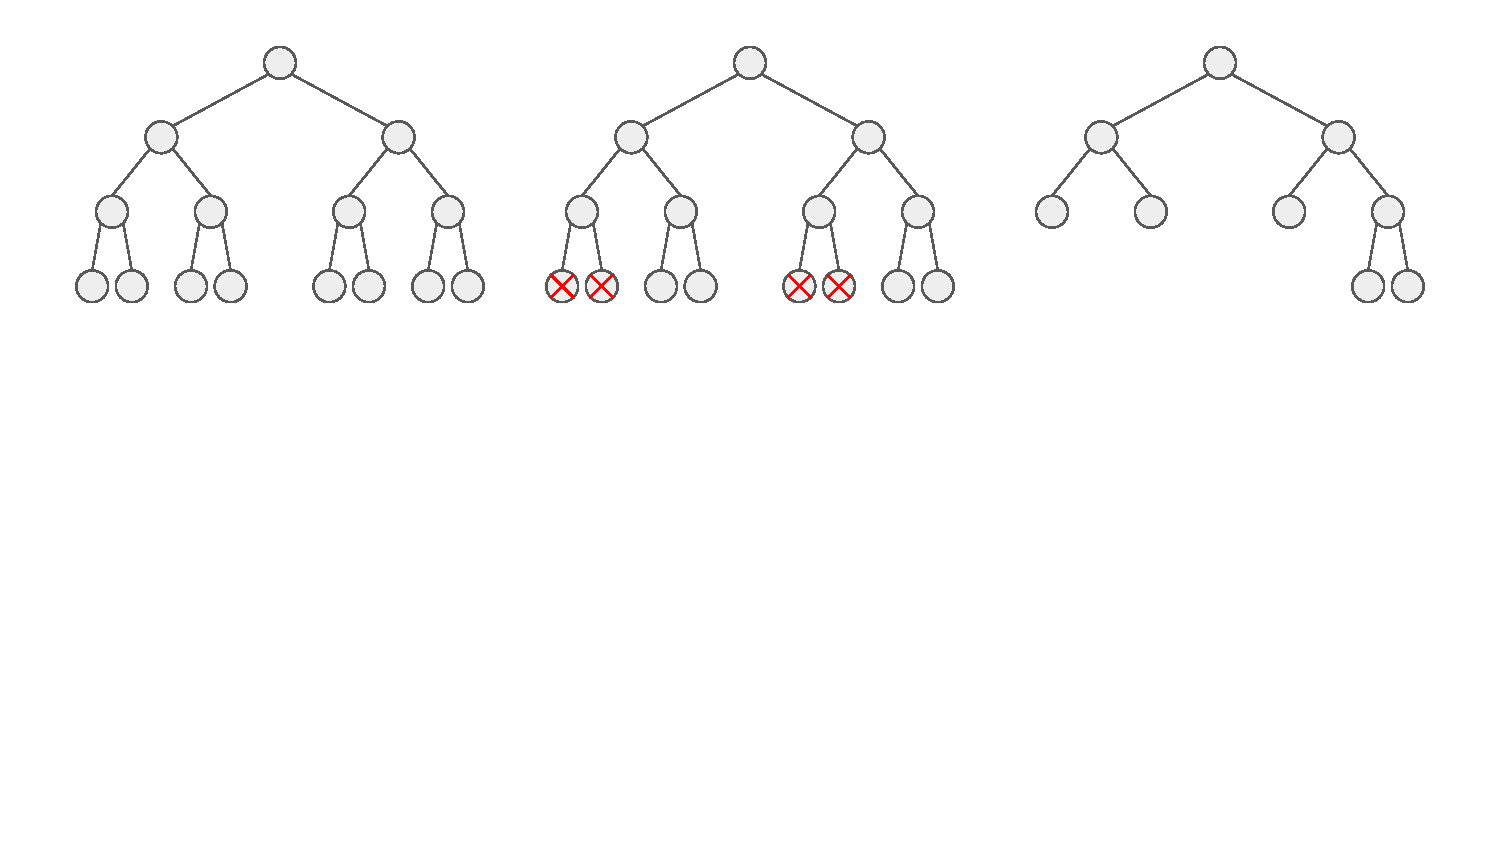
\includegraphics[trim=0 200 0 0, clip, width=\textwidth,page=1]{figure_man/trees_balance.pdf}
\caption{Tree with \texttt{max\_depth}=3. Balanced tree (left), pruned balanced tree (middle), leave-wise grown tree (right)}
\end{figure}

\end{vbframe}

\begin{vbframe}{Data Sampling: Gradient-based One-Side Sampling (GOSS)}

Recall: \pkg{XGBoost} use random data subsampling, i.e. stochastic gradient boosting.

\lz

Stochastic gradient boosting can be improved by \emph{smarter} sampling strategies based on the values of the gradients.

\lz

\textbf{GOSS:}
\begin{itemize}
  \item To evaluate a split GOSS only uses the $a\cdot n$ observations with largest (absolute) gradients and samples $b\cdot n$ observations from the remaining.
  \item The randomly sampled observations with smaller gradients are weighted by $\frac{1 - a}{b}$.
  \item Default values are $a=0.2$ and $b=0.1$.
  \item GOSS is only used after $\frac{1}{\nu}$ iterations of regular boosting steps.
\end{itemize}


\end{vbframe}

\begin{vbframe}{Data Sampling: Minimal Variance Sampling (MVS)}


\begin{itemize}
  \item MVS computes weights and selection probabilities of observations for a tree.
  \item The weighting is computed from the regularized absolute value $\hat{g}^{[m]}(\xi)=\sqrt{g^{[m]}(\xi)^2 + \lambda h^{[m]}(\xi)^2}$.
  \item Observations with a value of $\hat{g}^{[m]}(\xi) > \mu$ are always used and other observations are selected with probability $\frac{\hat{g}^{[m]}(\xi)}{\mu}$.
  \item $\mu$ has a closed-form nearly optimal solution for minimizing the risk of a tree base learner \textbf{(Ibragimov et al. 2019)}.
  \item For the tree fit each observation is weighted inversely proportional to its selection probability.
\end{itemize}

\lz

\textbf{Note:} $g^{[m]}(\xv) = \frac{\partial L(y, \fmd(\xv))}{\partial \fmd(\xv)}$ and $h^{[m]}(\xv) = \frac{\partial^2 L(y, \fmd(\xv))}{\partial {\fmd(\xv)}^2}$.

\end{vbframe}


\begin{vbframe}{Feature compression}

For high dimensional (sparse) data it can be helpful to bundle similar features together to speed up split computations.

\lz

\textbf{Exclusive feature bundling} looks for mutually exclusive features, i.e. features that never take nonzero values simultaneously.

\lz

\begin{itemize}
  \item A single histogram for approximate split finding in boosting can be built from multiple mutually exclusive features nearly without loss of information.
  \item Mutually exclusive features only occur in sparse data.
  \item This approach speeds up the histogram building from $\mathcal{O}(np)$ to $\mathcal{O}(nb)$ where $b$ is the number of feature bundles.
  \item While finding the optimal bundling is $np$-hard, greedy approximations give good results empirically.
\end{itemize}

\end{vbframe}

\begin{vbframe}{Categorical Features}

Even though \pkg{XGBoost} uses trees it does not support categorical features.

\lz

Both \pkg{LightGBM} and \pkg{CatBoost} provide \emph{target} encoding strategies for categorical features:

$$
  \tilde \xb_j = \frac{\sum_{i:\xb_j=l}y^{(i)}}{N_l}, \quad l=1,\dots,k
$$

where $N_l$ is the number of observations of the $l$'th level of categorical feature $\xb_j$.

\lz

Additional noise can added to the encoding to avoid overfitting for level with few observations.

\lz

Features with relatively few levels $k \le \tau_\text{max\_cat\_to\_onehot}$ (default $4$) are one-hot encoded.

\end{vbframe}


\begin{vbframe}{Feature Comparison of Boosting frameworks}

  \begin{scriptsize}

\begin{tabular}{lcccc}
  \toprule
   & Parallel & GPU Support & Approx. splits & Categ. feats\\
  \midrule
  XGBoost  & $x$ & $x$ & $x$ &     \\
  LightGBM & $x$ & $x$ & $x$ & $x$ \\
  CatBoost & $x$ & $x$ & $x$ & $x$ \\
  GBM      &     &     &     & $x$ \\
  H2O      & $x$ & $x$ & $x$ & $x$ \\
  sklearn  & $x$ &     & $x$ & $x$ \\
  \bottomrule
\end{tabular}

\lz

\begin{tabular}{lccccc}
  \toprule
   & \multicolumn{2}{c}{Tree growing} & \multicolumn{3}{c}{Subsampling} \\
  \midrule
            &        &               & \multicolumn{2}{c}{Observations} & Feats \\
            & Depth-wise & Leaf-wise & Regular & Gradient-based & \\
  \midrule
  XGBoost   & $x$ & $x$ & $x$ & $x$ & $x$ \\
  LightGBM  & $x$ & $x$ & $x$ & $x$ & $x$ \\
  CatBoost  & $x$ & $x$ & $x$ & $x$ & $x$ \\
  GBM       &     & $x$ & $x$ &     &     \\
  H2O       & $x$ &     & $x$ &     & $x$ \\
  sklearn   & $x$ &     & $x$ &     & $x$ \\
  \bottomrule
\end{tabular}

\end{scriptsize}

\end{vbframe}
\endlecture
\end{document}
